\documentclass{article}
 
\usepackage[T2A]{fontenc}
\usepackage[utf8]{inputenc}
\usepackage[russian]{babel}
\usepackage{titlesec}
\usepackage{amsmath}
\usepackage{amssymb}
\usepackage{algpseudocode}

\newcommand{\mathbbm}[1]{\text{\usefont{U}{bbm}{m}{n}#1}}

\usepackage{hyphenat}
\usepackage{graphicx}
\usepackage[left=2cm,right=2cm,
    top=2cm,bottom=2cm,bindingoffset=0cm]{geometry}
\hyphenation{ма-те-ма-ти-ка вос-ста-нав-ли-вать}

\newtheorem{theorem}{Theorem}
 
\title{Big Self-Supervised Models are Strong Semi-Supervised Learners: paper summary}
\author{Грачёва Анастасия}
 
\begin{document}
 
\maketitle

\section{Введение}
Обучение сначала на большом количестве неразмеченных данных в независимом от задаче виде, а затем дообучение на малом количестве размеченных данных - ещё недостаточно популярный в компьютерном зрении, но уже хорошо показавший себя в разметке на ImageNet метод. Оказывается, что в этом случае чем меньше процент размеченных данных, тем больше пользы извлекает модель от увеличения числа параметров. Этим данный метод отличается от обучения с учителем, при котором модели склонны к переобучению при увеличении числа параметров. После дообучения полученная модель может быть использована в качестве учителя для дистилляции в модель меньшего размера. При этом, её ответы на неразмеченных данных становятся <<разметкой>> для обучения модели-студента уже под конкретную задачу.

\section{Ключевые результаты}

\begin{itemize}
    \item При обучении с частичным привлечением учителя модель извлекает тем больше пользы из увеличения её размера, чем меньшее количество разметки используется. Зависимость проиллюстрирована на графике:
    
    
    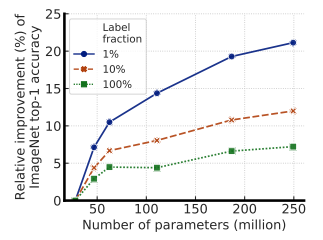
\includegraphics[scale=0.6]{1st_result.png}.
    
    
    \item Тем не менее, при переходе к обучению под конкретную задачу (разметки) размер модели можно уменьшить с небольшими потерями в качестве классификации, если использовать предсказания большой модели на неразмеченных данных.
    \item Показана важность проекционных слоёв после последовательности свёрточных, а также важность дообучения с середины этих слоёв.
    \item Предложена модель в совокупности с алгоритмом обучения - SimCLRv2, которая является улучшенной версией разработанной ранее SimCLR.
    \item SimCLRv2, основанная на ResNet-152, достигла точности 79.8\% на ImageNet, опередив предыдущего лидера в разделе обучения с частичным привлечением учителя на $\approx$4\%. Это результат т.н. <<линейной оценки>>, когда поверх полученных обучением без привлечения учителя представлений обучается линейный слой.
    \item Если проводить дистилляцию в модель того же размера (ResNet-152), то при дообучении на 1\% / 10\% данных получена точность 76.6\% / 80.9\%, что опережает предыдущие результаты более чем на 21 / 8 пунктов соответственно.
    \item Если же дистиллировать в меньшую модель (ResNet-50), то достигается точность  73.9\% / 77.5\% соответственно. Для сравнения, при стандартном обучении ResNet-50 с учителем на всех данных, это значение равно 76.6\%
    
    
    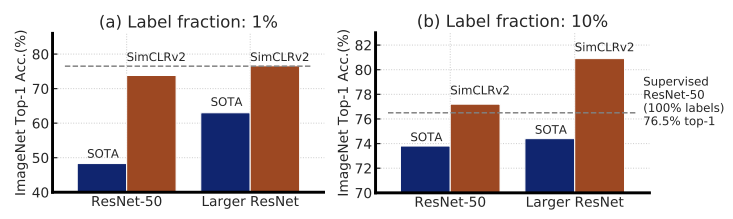
\includegraphics[scale=0.5]{leaderboard.png}.
    
    
\end{itemize}

\section{Метод}
SimCLRv2 выучивает представления, максимизируя согласие между различными аугментированными версиями одного и того же изображения с помощью контрастной функции потерь в пространстве скрытых представлений.
При обучении происходит следующее:
\begin{enumerate}
    \item Берётся случайно выбранный мини-батч изображений.
    \item Каждое из них аугментируется дважды с помощью случайной обрезки, искажения цвета и гауссовского размытия, создавая две версии одной  и той же картинки.
    \item Эти два изображения сначала проходят через свёрточную сеть на основе ResNet, а затем через несколько слоёв с нелинейностями, давая на выходе представления $z_i$  и $z_j$.
    \item Выходы затем используются для подсчёта контрастной функции потерь.
\end{enumerate}

Рассматривая мини-батч аугментированных примеров, значение функции потерь между парой примеров i, j, полученных из одного и того же изображения, можно задать следующим образом:

\begin{equation}
    \ell_{i,j} = -\log \frac{\exp(\mathrm{sim}(\bm z_i, \bm z_j)/\tau)}{\sum_{k=1}^{2N} \mathbbm{1}_{k \neq i}\exp(\mathrm{sim}(\bm z_i, \bm z_k)/\tau)}~,
\end{equation}
где $\mathrm{sim}(\cdot,\cdot)$ - косинусное сходство, а $\tau$ - <<температура>>.

Может возникнуть вопрос, почему во втором пункте используются именно такие аугментации изображения. На самом деле, в предыдущей статье (<<A Simple Framework for Contrastive Learning of Visual Representations>>) о модели SimCLR была проведена объёмная работа по сравнению качества моделей, обученных с различными комбинациями пар аугментаций, и искажение цвета в совокупности со случайной обрезкой оказались ключевыми в достижении хорошего результата.


\section{Заключение}

Авторы предложили трёхэтапный алгоритм обучения, благодаря которому им удалось добиться лидерства как в задаче выучивания векторных представлений изображения (которая оценивается дообучением линейного слоя), так и в задачах классификации с использованием 1\% или 10\% размеченных данных. Также они нашли следующую закономерность: модель извлекает тем больше пользы из увеличения её размера, чем меньшее количество разметки используется при обучении.


\end{document}
